% C. Research strategy 6 pages total
% 2. Innovation 0.5 page maximum
% 3. Approach 4.5 – 5 pages
% 2. Innovation. Explain how the application challenges and seeks to shift current research
% or clinical practice paradigms. Describe any novel theoretical concepts, approaches or
% methodologies, instrumentation or intervention(s) to be developed or used, and any
% advantage over existing methodologies, instrumentation or intervention(s). Explain any
% refinements, improvements, or new applications of theoretical concepts, approaches or
% methodologies, instrumentation or interventions.
% 3. Approach. Describe the overall strategy, methodology, and analyses to be used to
% accomplish the specific aims of the project. Unless addressed separately, include how the
% data will be collected, analyzed, and interpreted. Discuss potential problems, alternative
% strategies, and benchmarks for success anticipated to achieve the aims. If the project is in
% the early stages of development, describe any strategy to establish feasibility, and
% address the management of any high risk aspects of the proposed work. Point out any
% procedures, situations, or materials that may be hazardous to personnel and precautions
% to be exercised.
\section{Research Strategy}

\subsection{Significance}
% 1. Significance 0.5-1 page maximum
% C. Research Strategy. Must include Significance, Innovation, and Approach. For the first
% two sections, you can lump all aims into one Significance and one Innovation section
% (most popular choice) or you can repeat each section individually for each aim.
% Preliminary data can be included here if available.
% 1. Significance. Explain the importance of the problem or critical barrier to progress in
% the field that the proposed project addresses. Explain how the proposed project will
% improve scientific knowledge, technical capability, and/or clinical practice in one or
% more broad fields. Describe how the concepts, methods, technologies, treatments,
% services, or preventative interventions that drive this field will be changed if the
% proposed aims are achieved.



\begin{wrapfigure}{R}{0.5\textwidth}%{4.5cm}%靠文字内容的左侧
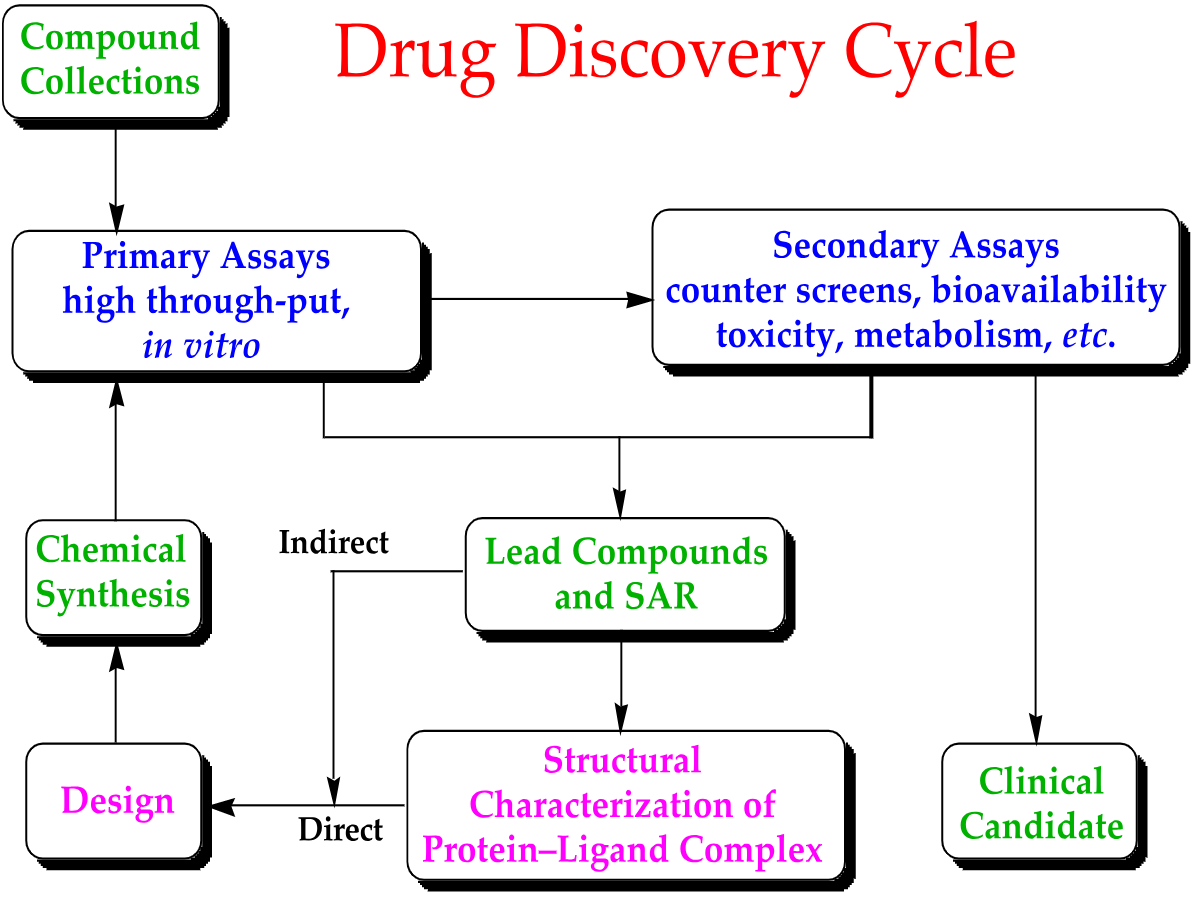
\includegraphics[width=0.49\textwidth]{../figures/wiki_drug.png}
\caption{Drug development steps\cite{wiki_drug}}
\label{fig:wiki_drug}
\end{wrapfigure}

Drug development is a very time-consuming and expensive process. %\cite{Carpenter2018}
Of the drug development pipeline as indicated in figure \ref{fig:wiki_drug}, 
while each of these steps are very much time and capital consuming,
these are inevitable steps that a putative drug has to go through to eventually make it to the market. 
Recently with the advent of computer science, much effort has been put into \textit{in silico} to aid the `Primary Assays high through-put, \textit{in vitro}' step as shown in figure \ref{fig:wiki_drug}.
As a main contribution brought by the growth of computing powers,
virtual screening is the alternative of actual physical high throughput screening (HTS).

Virtual screening is  defined as `automatically evaluating very large libraries of compounds using computer programs'.
With the ever growing size of databases of proteins (targets) and compounds (drug candidates),
A crucial drug identification step can be described as,
given a protein that is known to be closely related to a disease that is desired to be cured,
of the database of small molecules, which can be a potential drug candidate?

As a solution to the scenario described above, much efforts has been put into virtual screening that aims to identify a reliable drug hit that can be put into the drug development pipeline that eventually get optimized to a commercial drug (also known as hit-to-lead, lead-to-drug).

Among the efforts of developing virtual screening methods, one most popular model is structured-based drug design.
In structure based drug design, the structure (3D coordinates) of the ligand and receptor is known via other analyzing methods such as X-ray crystallography, NMR or homology modeling \cite{blundell1996structure}. 
Structure-based drug design mainly comprise of molecular docking studies. Given the nature of diseases that most involves the malfunction of enzymes and other forms of proteins, protein-ligand docking is of special interest among other docking types (protein-protein, protein-DNA etc.).
 
This proposal focuses on the improvement of virtual screening via the molecular docking and ligand selection method. Which, if proven to be functional, has the potential of applying to many other receptors that are yet to find the perfect drug.

% \begin{wrapfigure}{L}{0.4\textwidth}%{4.5cm}%靠文字内容的左侧
% 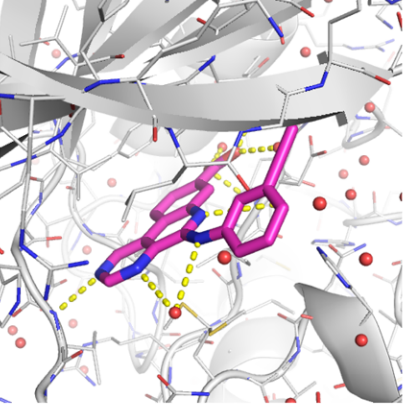
\includegraphics[width=0.38\textwidth]{../figures/docking_example.png}
% \caption{An example of docking (PDB ID: 3PE2) of a complex with it's naturally co-crystallized ligand \cite{Ragoza2017}}
% \label{fig:docking_example}
% \end{wrapfigure}

% The docking problem can be described as the search for the precise ligand conformations and orientations (also referred to as posing) within a given targeted protein when the structure of the protein is known.
% Figure \ref{fig:docking_example} shows are example of how a ligand is `docked' onto a target.
% The binding affinity prediction problem addresses the question of how well the ligands bind to the protein (scoring). 
% Therefore, the general docking program would include two subsequent parts: a searching algorithm and a scoring function. While the searching problem is relatively well resolved with random or stochastic algorithms \cite{Rezacova2008}, 
% on going efforts are still being put into developing a more accurate scoring function, as the current scoring functions incorporated inside of the mainstream docking softwares such as DOCK\cite{dock}, AutoDock\cite{autodock}, GOLD\cite{gold}, Glide\cite{glide}, and Surflex-Dock\cite{surflex}.
% While the average drug company has a wide choice of docking software to choose from, 
% there's no agreement of one single scoring functions outperforms the rest, 
% despite of whether it's academically free or commercially expensive.
% In fact, depending what architecture or training data set (for empirical based scoring functions) per scoring function is using, 
% one scoring function tend to perform better for certain protein-ligand docking types.
% And it is often the case that certain compounds are identified via virtual screening to be a `binder' while subsequent experimental results show that it's not.
% Such misidentifying events are undesired and are to be minimized through the efforts towards better virtual screening results. Therefore it's an ongoing effort to design better scoring functions.

% \rep[inline]{Rephrase stuff in reference to this paragraph:Scoring functions are typically classified into three groups: force field, knowledge-based and empirical. Force field scoring functions parameterize the potential energy of a complex as a sum of energy terms arising from bonded and non-bonded interactions (Huang et al., 2006). The functional form of each of these terms is characteristic of the particular force field, which in turn contains a number of parameters that are estimated from experimental data and computer simulations. These force fields were designed to model intermolecular potential energies, and thus do not account for entropy (Kitchen et al., 2004). Knowledge-based scoring functions use the 3D co-ordinates of a large set of protein–ligand complexes as a knowledge base. In this way, a putative protein–ligand complex can be assessed on the basis of how similar its features are to those in the knowledge base. The features used are often the distributions of atom–atom distances between protein and ligand in the complex. Features commonly observed in the knowledge base score favourably, whereas less frequently observed features score unfavourably. When these contributions are summed over all pairs of atoms in the complex, the resulting score is converted into a pseudo-energy function, typically through a reverse Boltzmann procedure, in order to provide an estimate of the binding affinity (e.g. Gohlke et al., 2000; Mitchell et al., 1999a, b; Muegge and Martin, 1999; Konstantinou Kirtay et al., 2005). Some knowledge-based scoring functions now include parameters that are fitted to experimental binding affinities (e.g. Velec et al., 2005) or introduce Information Theory-driven improvements as well as explicit solvent models (Kulharia et al., 2008). Lastly, empirical scoring functions calculate the free energy of binding as a sum of contributing terms, each identified with a physicochemically distinct contribution to the binding free energy such as: hydrogen bonding, hydrophobic interactions, van der Waals interactions and the ligand's conformational entropy. Each of these terms is multiplied by a coefficient and the resulting parameters are estimated from binding affinities. In addition to scoring functions, there are other computational techniques, such as those based on molecular dynamics simulations, that provide a more accurate prediction of binding affinity. However, these expensive calculations remain impractical for the evaluation of large numbers of protein–ligand complexes and are currently typically limited to family-specific simulations (Guvench and MacKerell Jr, 2009; Huang et al., 2006).Scoring functions do not fully account for a number of physical processes that are important for molecular recognition, which in turn limits their ability to select and rank order small molecules by computed binding affinities. It is generally believed (Guvench and MacKerell Jr, 2009) that the two major sources of error in scoring functions are their limited description of protein flexibility and the implicit treatment of solvent. }


\subsection{Innovation}

\begin{wrapfigure}{L}{0.4\textwidth}%{4.5cm}%靠文字内容的左侧
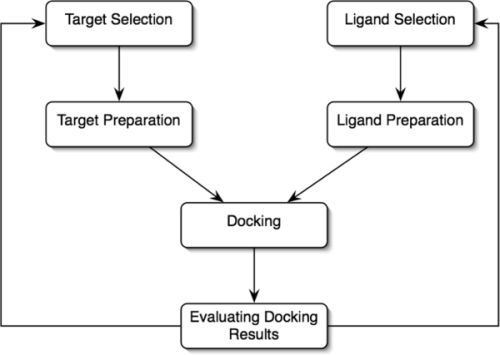
\includegraphics[width=0.385\textwidth]{../figures/docking_flow.png}
\caption{General docking steps\cite{Morris2008}}
\label{fig:docking_flow}
\end{wrapfigure}

The general process of structure based virtual screening can be briefly described as below: 
\begin{quotation}
Identify the protein of interest as target, prepare a library of ligands that is to be screened, perform molecular docking on each one of the ligand and evaluate the binding affinity of each protein-ligand pair and decide with ligands are to be used for subsequent optimization (hit to lead) and bioassay.
\end{quotation}
Despite the fact that there are a variety of molecular docking softwares, and much effort has been putting into building more accurate scoring functions for predicting binding affinities, 
the execution of molecular docking in the virtual screening scenario is often \textit{using the default docking parameters}. 

The innovation of aim \Romannum{1} will be to build a predictor for generating docking parameters that's tuned to the ligand molecule. The `predictor' is build via a SVM algorithm, in which the training dataset will be generated from an evaluating protocol.

Aim \Romannum{2} focuses on increasing the efficiency of screening,
as opposed to `go through' the ligand library and perform molecular docking one by one, 
every ligand that has been docked will be labeled as `binder' or `non-binder', along with the untested ligands, the ligand library will be projected to a higher space and and the labeled data will serve to help choosing what ligand to dock next.
As the screening goes the amount of labeled data will grow as well, hence this is an active learning process in terms of ligand selection.

Aim \Romannum{1} and \Romannum{2} combined will be implemented in finding a hit for Alzheimer's disease (AD) related targets in aim \Romannum{3}. AD is a neurodegenerative disease with no known cure and prevention. 



% This article propose a machine learning architecture for molecular docking methodology.
% Molecular docking is the critical step in structure based drug design in virtual screening.
% A frustration situation in todays \textit{in silico} screening 
% is that
% drug leads that are predicted to be active binder of the target protein 
% fail to bind in real experimental conditions.
% Generally it is summarized this is due to the limitations of the docking software,
% more specifically, the scoring functions within the docking software.
% Scoring functions have been under active development towards better estimation of binding affinity,
% and much efforts have been put into building more realistic model in molecular dynamics level, 
% or incorporating machine learning algorithms training towards better predicting scoring functions.
% However, not much efforts are put into a complex-specific configuration per docking event.
% This article uses the CASF scoring functions evaluation protocol 
% to optimize the complex specific docking configuration
% with simple machine learning design.

\subsection{Approach}

\subsubsection{General description}

In structure based virtual screening, the key step is molecular docking. 
Molecular docking addresses two problems, the docking problem and the binding affinity prediction problem.
The docking problem can be described as the search for the precise ligand conformations and orientations (also referred to as posing) within a given targeted protein where the structure of the protein is known.
The binding affinity prediction problem addresses the question of how well the ligands bind to the protein (scoring). 

Therefore, the general docking program would include two parts: 
a searching algorithm and a scoring function. 
While the searching problem is relatively well resolved with random or stochastic algorithms \cite{Rezacova2008}, 
on going efforts are still being put into developing a more accurate scoring functions. 
Up until now, many scoring functions based on different methodology have been developed, currently a range of different scoring functions have incorporated inside of the mainstream docking softwares such as DOCK\cite{dock}, AutoDock\cite{autodock}, GOLD\cite{gold}, Glide\cite{glide}, and Surflex-Dock\cite{surflex}.

Of the various model type of scoring functions out there which are traditionally categorized into force-field-based, empirical, knowledge- based, 
with each of the categories has it's strengths and weaknesses.
Shortly, with the approximation researchers have to adopt in some models, or, limitation of the training set sizes for building the model, 
it is summarized that no single docking program has dominative advantages than other programs.\cite{wang2016}.
While the average drug company has a wide choice of docking software to choose from, 
there's no agreement of one single scoring functions outperforms the rest, 
despite of whether it's academically free or commercially expensive.

In fact, depending on what architecture or training data set (for empirical based scoring functions) per scoring function is using, 
one scoring function tend to perform better for certain protein-ligand docking types.
And it is often the case that certain compounds are identified via virtual screening to be a `binder' while subsequent experimental results show that it's not.

With the advent of computational power, there has been a trending of implementing machine learning algorithm into molecular docking, thus given the forth category of `machine-learning based' or `descriptor-based' scoring function. 
Based on the fact that molecular docking problem can be described as building a model with a known-to-bind data sets that can be treated as the training sets, which suits into the category of supervised-learning in machine-learning concepts, multiple algorithm including Na\"{i}ve Bayes, k-Nearest Neighbors, Support Vector Machine, Random Forests and Artificial Neural Networks \cite{Carpenter2018}.

While machine learning could be a powerful tool, 
the current architecture of using machine learning in the molecular docking field either be viewed as `black box feature selection' \cite{Gabel2014} with the danger of over fitting training data, 
or has complicated feature parameters\cite{Lo2018}. 

In aim \Romannum{1}, machine learning will be used in combination with a traditional scoring function (specifically, smina will be used to illustrate the data flow, but it can be any other scoring function of with enough user defined flexibility).
Shortly, after a normal `docking' performed by smina, 
docking parameters will be updated iteratively until it passes the CASF protocol on a user defined threshold.
Subsequently molecular descriptors will be generated corresponding to the optimized docking configuration, 
a machine learning algorithm (SVM) will learns the relationship between the descriptors and the docking configurations. The general logic flow is illustrated in figure \ref{fig:flow}, the specific terms that appear in this flow chart will be explained in later sections.

\begin{figure}[htbp]
\centering
\begin{tikzpicture}[node distance = 2cm, auto]
    % Place nodes
    \node [block] (init) {PDBbind coreset};
    \node [block, below of=init] (identify) {receptor + ligand + config};
    \node [block2, right of=identify, node distance=3cm] (md) {molecular descriptor};   
    \node [block, below of=identify, node distance=3cm] (evaluate) {smina: docking and scoring};
    \node [block, left of=evaluate, node distance=3cm] (update) {update config};
    \node [decision, below of=evaluate] (decide) {pass the CASF protocol?};
    \node [block, below of=decide, node distance=3cm] (stop) {stop};
     \node [block2, right of=stop, node distance=3cm] (config) {config};
     \node [block3, below of=md, node distance=3cm] (svm) {svm};
    % Draw edges
    \path [line] (init) -- (identify);
    \path [line] (identify) -- (evaluate);
    \path [line] (identify) -- (md);
    \path [line] (evaluate) -- (decide);
    \path [line] (decide) -| node [near start] {no} (update);
    \path [line] (update) |- (identify);
    \path [line] (decide) -- node {yes}(stop);
   \path [line] (md) -- (svm);
   \path [line] (config) -- (svm);
   \path [line] (stop) -- (config);
\end{tikzpicture}
\caption{Systematic illustration of the proposed algorithm}
\label{fig:flow}
\end{figure}


Aim \Romannum{2} steps back to look at virtual screening in a bigger picture.
The size of small molecular library is usually on the order of thousands even after pre-filtering. It's natural to dock one by one with random order, but a selective method promises to be more time efficient if the amount of binders are predetermined.
Again, a machine learning method is used in this step.

Finally, aim \Romannum{3} proposes the application of the architecture to a realistic scenario of Alzheimer's disease. 
While AD itself is notoriously famous for complicity of cause and different hypothesis for treatment, this proposal focuses on the amyloid cascade hypothesis 
in which acetylcholinesterase (AChE) is targeted using small molecule inhibitor.



\subsubsection{Choice of molecular docking software: Smina} 

To provide some background information, 
AutoDock \cite{autodock} is one of the most cited docking software, 
and AutoDock Vina  \cite{vina} is the improved docking software in which the fundamental model of scoring was improved and has since become the popular academical docking software.

In a typical docking event, the docking software would take in the respective structure file of the ligand and the receptor, along with the instruction of docking specific parameters and performs pose searching and binding affinity calculation subsequently \cite{Diederichs2016}. 
With any docking software (not just Vina), the parameters must include a minimum of search space, 
but optional parameters can be specified, take Vina for example, the additional specifications can be:
\begin{itemize}
	\item seed: random seed for where to start sampling inside of the search box
	\item exhaustiveness: how much should the sampling algorithm explore into different binding poses
	\item num\_modes: how many most optimized poses the user want Vina to output
	\item energy\_range: maximum energy difference between the best binding mode and the worst one displayed in units of kcal/mol
\end{itemize}
The search space would ideally be the minimum box that contain the protein's natural co-crystallized ligand, but the larger it is, the more searching Vina will have to do.

Despite the face that Vina offers `tweaking' of the starting conditions, 
it doesn't provide much user-defined functionality as in which of the bonds or side chains are flexible.


Note that, there are multiple (more than 50) docking softwares out there for virtual screening, 
the choice of smina is based on it's versatility for instructing per given protein ligand docking event as described above.
Below shows an example of how smina can be `tweaked' to allow for different docking configurations (which the authors refer to as `versatile scoring function').


\begin{lstlisting}[language={},caption = smina user defined parameters, frame=single, label = smina]
1.0  ad4_solvation(d-sigma=3.6,_s/q=0.01097,_c=8)  desolvation, q determines whether value is charge dependent
1.0  ad4_solvation(d-sigma=3.6,_s/q=0.01097,_c=8)  in all terms, c is a distance cutoff
1.0  electrostatic(i=1,_^=100,_c=8)	i is the exponent of the distance
1.0  electrostatic(i=2,_^=100,_c=8)
1.0  gauss(o=0,_w=0.5,_c=8)		o is offset, w is width of gaussian
1.0  gauss(o=3,_w=2,_c=8)
1.0  repulsion(o=0,_c=8)	o is offset of squared distance repulsion
1.0  hydrophobic(g=0.5,_b=1.5,_c=8)		g is a good distance, b the bad distance
1.0  non_hydrophobic(g=0.5,_b=1.5,_c=8)	value is linearly interpolated between g and b
1.0  vdw(i=4,_j=8,_s=0,_^=100,_c=8)	i and j are LJ exponents
1.0  vdw(i=6,_j=12,_s=1,_^=100,_c=8) s is the smoothing, ^ is the cap
1.0  non_dir_h_bond(g=-0.7,_b=0,_c=8)	good and bad
1.0  non_dir_h_bond_quadratic(o=0.4,_c=8) like repulsion, but for hbond, don't use	
1.0  non_dir_h_bond_lj(o=-0.7,_^=100,_c=8)	LJ 10-12 potential, capped at ^
1.0 acceptor_acceptor_quadratic(o=0,_c=8)	quadratic potential between hydrogen bond acceptors
1.0 donor_donor_quadratic(o=0,_c=8)	quadratic potential between hydroben bond donors
1.0  num_tors_div	div constant terms are not linearly independent
1.0  num_heavy_atoms_div	
1.0  num_heavy_atoms	these terms are just added
1.0  num_tors_add
1.0  num_tors_sqr
1.0  num_tors_sqrt
1.0  num_hydrophobic_atoms
1.0  ligand_length
\end{lstlisting}

Conveniently the \texttt{1.0} s are weights to be put into consideration when docking. 
Taking out the parameters that are not optimizable, but rather, rely on the property of the receptor and the ligand, the optimizable weights will be optimized in an iterative style.
For each ligand-receptor complex, the end goal is to construct a vector containing the optimal docking parameters (weights) associated with it.

\subsubsection{Usage CASF evaluation protocol for optimizing docking parameters} \label{CASF}

The default vector in smina, if not user defined, will be a vector of ones. 
We aim to tune it to a more complex-specific vector which potential gives better binding affinity prediction. This process will be phrased as `optimizing docking parameters'.
To optimize the docking parameters, we propose to use the CASF evaluation protocol.

Generally, scoring functions are evaluated in the context of molecular-docking trials.
Specifically, evaluation of the performance of scoring functions in dicking has focused predominantly on two measure. 

First, the ability to accurately reproduce the co-crystallized ligand binding poses in crystal structures, it is arbitrarily defined that ligand docking is most accurate if the top ranked pose has a heavy atom root mean square deviation (RMSD, atomic positions as the measure of the average distance between the atoms of superimposed proteins) less than $2\si{\angstrom}$ from the location of the crystallized ligand.
Second, the enrichment factor (EF) of the docking and soring algorithm after a virtual screening event. The EF is defined as the accumulated ratio of active ligands found above a certain percentile of the ranked database containing active and inactive ligands ('binders' and `non-binders'). A higher EF value at the define percentile normally indicates a better scoring function.
Another evaluation that is less frequently exercised is the accuracy in prediction of the experimental binding affinity, even though this was the original definition for scoring functions in molecular docking.
This is not only because of the inability of the current scoring functions available, but also the data quality deposited in the protein data bank by various researchers not following a universally experimental condition when performing the data acquisition.

To date, several publications has addressed the performance of scoring functions by comparison studies. 
while the general capabilities described above are covered, 
there hasn't been a universal benchmark until March, 2018, When \citet{li2018assessing} introduced a
protocol in which the capabilities of one given scoring function is summarized into four indicators: scoring power, ranking power, docking power and screening power.
\citet{li2018assessing} also introduced the CASF benchmark datasets where the evaluation of the datasets are parameterized and described as `a common language among the scoring function community'.

There are currently more than 35,000 crystallographic or NMR structures of proteins or nucleic acids available from the Protein Data Bank (PDB) \cite{Bernstein1977}. 
PDBbind is database is a comprehensive collection of the experimentally measured binding affinity data 
for all types of biomolecular complexes deposited in the PDB\cite{wang2004pdbbind}.
The CASF benchmark \cite{li2014comparative} is development upon PDBbind, 
including a high quality data set and quantitative methods for conducting performance evaluation.

The actual complex dataset that the performance of the scoring functions will be evaluated on will be referred to as `core set'. 
The core set consists of 195 protein-ligand complexes in 65 protein clusters.
It is designed to cover protein-ligand complexes formed by diverse proteins 
so that they can be representative of the target-to-be in a real virtual screening situation.
The complexes in the core set are chosen such that they have a reliable crystal structure and experimental binding data, and they are also chose to be drug relevant in the sense that most (82\%) of the ligand molecules are evaluated to obey the Lipinski's `rule of five' as the primary filter for drug-likeness, and the majority of proteins (78\%) are validated as potential drug candidate.
Most importantly, the 195 complexes can be categorized into 65 clusters with each cluster containing a representative of 3 complexes that span nearly 10 orders of magnitude in binding affinity (Kd = 10 mM – 1 pM).

On top of the high quality data set, the CASF benchmark define the power of a scoring function as scoring power, ranking power, docking power and screening power.
While the original intention of a `scoring' function is to estimate the binding affinity of a given protein and ligand pair, the practical application scenario is far more complicated, in addition to the fact that scoring functions are modules that are incorporated inside of molecular docking softwares, 
while the software relies on the scoring function on the most part for predicting a binding affinity, it also contains a searching function (pose sampling) functionality prior to determine 1. active site of the target protein 2. binding pose of the given ligand.
Therefore, to just evaluate on the scoring function, it is necessary to decouple these variable from the scoring function, in which case the decoy ligand-binding poses for each complex is to be generated in advance and the scoring functions will be instructed to predict a binding affinity based on the decoy poses.
% the
% decoy ligand-binding poses for each complex were generated in advance. This is one of the key ideas of our CASF benchmark. To prepare the decoy ligand-binding poses, we

The `powers' of per given scoring functions are defined as follows according to the CASF protocol.
\begin{itemize}
	\item Scoring power: the capability to produce binding score in linear correlation with experimental bind data. Quantitatively, by Pearson correlation coefficient (R) and the standard deviation between predicted and experimental. 
	\item Ranking power: the capability of rank the ligands of a given target protein correctly with given binding pose. Quantitatively, define a `success rate' of $\frac{correct~ranking~sets}{overall~ranking~sets}$.
	\item Docking power: the capability to identify the native ligand-binding pose among computer generated decoy poses. Quantitatively, if the RMSD value between the native binding pose from the top-ranked binding pose fell below a predefined cutoff.
	\item Screening power: capability to identify true binders for a given target protein among a pool of random molecules. Here define enhancement factor (EF) defined as below: (1\% can~be~set~to~other~user~defined~threshold)
	\begin{equation*}
	EF_{1\%} = \frac{number~of~true~binders~among~top~1\% candidates}{(total~number~of~true~binders~for~this~target~protein) \times 1\%} 
	\end{equation*}
\end{itemize}

To fit CASF protocol into the optimizing step, all of the 195 data will be docking using initial docking parameter (the vector of ones) and the initial powers of smina will be evaluated. 
We propose to set the `passing threshold' be 10 percent more (can be changed practically in view of computational time) than the initial powers, and the docking parameters will be updated and re-evaluated after each update.

CASF protocol provide bash scripts that runs and output numbers as the representation of each of the powers and the outliers will be updated first.
For each `update of parameters', a simple gradient descent algorithm will be used.


\subsubsection{Generating molecular descriptors}
% A descriptor-based scoring function usually consists of a considerably larger number of descriptors than an empirical scoring function. It is unclear if one can always obtain a converged model if different sets of descriptors are supplied as the input for machine learning. Second, an empirical scoring function adopts a theory-inspired functional form that is predetermined by human; whereas a descriptor- based scoring function relies on machine-learning technique to select the final model. The individual terms in an empirical scoring function normally have interpretable physical meanings; while in the case of a descriptor-based method, the rationale for selecting a certain combination of descriptors is often vague. In this sense, a descriptor-based scoring function is essentially a
% “black box” as many QSAR models
Molecular descriptor is a necessity in view of converting molecular to `computer language', 
it will serve as the input of any machine learning algorithm.
Shortly, molecular descriptors are numerical values assigned to structures,
they can be physiochemical properties (molecular weight, logP), 
or more sophisticated indicators such as topological indices, maximum common substructures, molecular fields\cite{todeschini2008handbook}.

Usually, the actual `molecular descriptor' utilized in machine learning scenarios are more complicated than what's described above, and there's are novel algorithms that doesn't not rely on simple linear descriptors (sun as constitutional neural network \cite{Ragoza2017}). 
To show a illustrative example of how molecular descriptors as numerical matrices can be used describe the molecular itself, consider an example based on elemental atom types as shown below: \cite{Ballester2012}

For both the protein P and the ligand L:
\begin{equation*}
\{ P(j)\}_{j=1}^9 = \{C,N,O,F,P,S,Cl,Br,I\}~~~~\{L(i)\}_{i=1}^9 = \{C,N,O,F,P,S,Cl,Br,I\}
\end{equation*}
The occurrence count for a particular j-i atom type pair is defined as:
\begin{equation*}
\varkappa _{Z(P(j)),Z(P(i))} \equiv \sum_{k=1}^{K_j} \sum_{l=1}^{L_i} \Theta (d_{cutoff}-d_{kl})
\end{equation*}
where $d_{kl}$ is the Euclidean distance between $k-th$ protein atom of type $j$ and the $l-th$ ligand atom of type $i$ calculated from the PDBbind structure.
$K_j$ is the total number of protein atoms of type $j$ and 
$L_i$ is the total number of ligand atoms of type $i$ in the considered complex;
$Z$ is a function that returns the atomic number of an element and it is used to rename the feature.
$\Theta$ is the Heaviside step function that counts contacts within a defined cutoff.
For example, when $d_{cutoff}=12\si{\angstrom}$ it means that it counts the atoms within a $12 \si{\angstrom}$ neighborhood of the given atom.

This is an simplified illustration of the most prevailed machine learning descriptors 
that rely on a pair-wise feature selection.
Depending on the end users' intension, there are many ready to use commercial softwares that generate numerical descriptors for machine learning input.

In this proposal, Dragon will be used for generating the molecular descriptors.
The choice of based on that fact that Dragon is able to calculate 5270 molecular descriptors, covering most of the various theoretical approaches.
Of the descriptors that Dragon offers to calculate, choice will be made among the 
\textit{3D Atom Pairs}, \textit{3D matrix-based descriptors} , \textit{Topological indices} descriptors as these will mostly likely to be relevant.

\subsubsection{SVM for learning the relationship between docking parameters and ligand molecular descriptors} \label{svm}

\begin{wrapfigure}{R}{0.48\textwidth}%{4.5cm}%靠文字内容的左侧
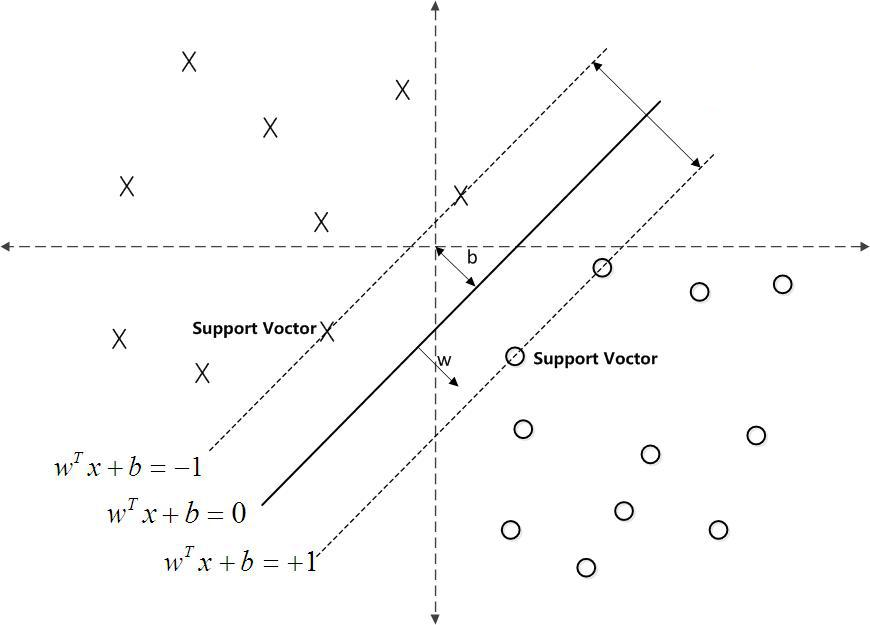
\includegraphics[width=0.445\textwidth]{../figures/svm_intro.png}
\caption{Illustration of how SVM multi-class classification on a data set with different kernel functions\cite{svm_sklearn}}
\label{fig:svm}
\end{wrapfigure}

The simplicity of this proposal is that it uses well-built machine learning structure instead of building a model that involves the very tedious molecular dynamics model building which is not just time consuming, but also computationally expensive \cite{Lo2018}.

To this point, we have described the input for SVM, which will be a vector that specifies the docking parameter, and the corresponding molecular descriptor. 
And we will have this information for all of the 195 complexes.

Below offers a short description of SVM that will be trained will the dataset described above to serve as a predictor that per given molecular descriptor, it outputs the optimal docking parameters.

SVM is chose as the machine learning algorithm based on the advantages below: \cite{svm_sklearn}
\begin{itemize}
	\item Effective in high dimensional spaces.
	\item Still effective in cases where number of dimensions is greater than the number of samples.
	\item Uses a subset of training points in the decision function (called support vectors), so it is also memory efficient.
	\item Versatile: different Kernel functions can be specified for the decision function. Common kernels are provided, but it is also possible to specify custom kernels.
\end{itemize}

Before illustration of how the versatility of the kernel functions possible greatly suits the need of this proposal, here is a brief introduction of how SVM works.

In SVM, each data item is plotted as a point in n-dimensional space (where n is the number of features predetermined) with the value of each feature being the value of a particular coordinate. Then classification is performed by finding the hyper-plain that differentiate the two classes.
SVM can be used for regression instead of classification with minor differences in which the hyper-plane needs to be individualized.
The function that projects the input data into the feature-dimension space is defined as a kernel function. 
The choice of the suitable kernel function can be crucial to the success of the training as shown in figure \ref{fig:svm}.
It is often suggested that the kernel function be chosen based on prior knowledge of the dataset.
As this case is mostly likely a non-linear model, the Radial Basis Function kernel would be used as the default and would be updated if needed.

Practically, the 195 datasets will be divided into 3 subsets, with mixed binding affinities in each sets. For training and testing, the leave-one-out cross validation method will be used.

\subsubsection{Aim \Romannum{2}: active selection of next ligand}

In the virtual screening pipeline, the simplest selection strategy is to choose new compounds at random for testing. 
It's intuitive that with random selection, the number of hits grows linearly with the total number of compounds that have been tested.
Since that most of the compounds will likely to be `non-binder', this random selection will be a very inactive process.

\citet{warmuth2003active} suggested an active learning with SVM will be employed in the virtual screening pipeline in this proposal. 
Refer to figure \ref{fig:svm} in section \ref{svm} for the concept of SVM.
Practically, all of the ligands to be screened will be projected in the feature space, 
a hyperplane will be calculated in this feature space to separate the known binders and non-binders with minimized cost.
And the ligand to be docked next will be the data point that's furtherest away from this hyperplane on the binder's side. It's intuitive that this data point is most likely to be categorized as a binder. 
This selection method is refer to as `active learning' because as the screening goes, the number of labeled data grows and the hyperplane is updated dynamically.

While this active learning selection strategy has be previously described in \citet{warmuth2003active}, it was never incorporated in the virtual screening event. 
The SVM algorithm that people utilized nowadays refers to the direct relationship of binders and the compound database without the step of molecular docking, in other words, SVM substitutes the molecular docking as the evaluation for binding affinity.


\subsubsection{Validation of the proposed virtual screening architecture: DUD$\cdot$E}

DUD$\cdot$E is full named as `a database of useful decoys: enhanced.' \cite{mysinger2012directory}, as the name suggests, it is an enhanced version of the previously prevailed DUD (directory of useful decoys).
It is designed to help benchmark molecular docking programs by providing challenging decoys.
It contains 22,886 active compounds and their affinities against 102 targets, an average of 224 ligands per target 50 decoys for each active having similar physico-chemical properties but dissimilar 2-D topology.

We will perform simulated virtual screening using this DUD$\cdot$E benchmark datasets, and before\& after ROC, AUC graphs will be plotted to evaluate the efficiency of the proposed architecture.


\subsubsection{Aim \Romannum{3}: applicate the combined docking software in virtual screening of drug lead for Alzheimer’s Disease}

This section aims to applicate the combined new scoring function to the classical virtual screening (VS) scenario.
Specifically, a small molecular library is run through with the combined virtual screening architecture.

Alzheimer’s disease (AD) is the most common form of dementia in the elderly with progressive cognitive decline and memory loss, 
it affects 44 million people worldwide as of 2016 \cite{winblad2016defeating}.
Unfortunately, AD and other neurological diseases are notoriously difficult to treat. 
The AD drugs currently available only alleviate symptoms\cite{schneider2011lack} and it is imperative to keep searching for a cure as in the most recent AD related drug to pass clinical trials (Memantine) happened in 2003.

Although there are many mechanisms for AD, it is generally agreed that there are only two classes of drugs currently available for AD treatment. 
This proposal will focus on acetylcholineterase inhibitors (AChEI), which increase acetylcholine concentration in cholinergic gynaptic clefts.

Primarily, BACE1, the M1 subtype of mAChR, APP, CDK5, and GSK-3$\beta$ are the potential targets \cite{Carpenter2018}.
And ZINC \cite{irwin2005zinc}  small compound library will be screened for potential drug hits.

Several recently studies have been done in search of AChEI \cite{fang2015discovery,chen2015discovery,kumar2017physicochemical,xie2017designing,ma2010silico}, while only \cite{fang2015discovery} used a machine learning based virtual screening. It would be mostly interesting to compare the filtered ligand results with the studies shown above.
% As AD is a polygenic and multifactorial disease with complex ori-
% gins, there is not an obvious target to choose. AD is characterized by aggregations of amyloid-beta (Aβ) plaques and neurofibrillary tangles (NFT) comprised of hyperphosphorylated tau protein [91, 92]. AD-affected brains also show a significantly reduced concen- tration of the neurotransmitter acetylcholine (ACh) [93, 94]. These two facts have sparked the main hypotheses around which AD treatments are based: the amyloid cascade hypothesis (the idea that the cognitive decline present in AD is caused by Aβ plaques) and the cholinergic hypothesis (the idea that it is caused by ACh loss). Early attempts to design an AD drug focused on the cholinergic hypothesis. Because of this, most existing AD treatments are cho- linesterase inhibitors. However, since these drugs are all palliative and do not stop neurodegeneration, AD drug design going forward is paying more attention to the amyloid cascade hypothesis.


\subsubsection{Concluding remarks}

% This proposal takes advantage of many open-source structures maturely built 
% but implement them onto a standards to assist better scoring capabilities of any scoring function given.
% It is theoretically relative simple to accomplish and has the potential of locating better lead for some protein targets.
This proposal builds upon currently available resources and construct machine learning architecture in a simple design, and applicates the architecture the ongoing search of AChEI.

The methodology is straightforward yet involved a traditionally robust machine learning algorithm, in future research can be applicate to the search of hits for other proteins as well.
